\section{Introduction \& background}
\lettrine[lines=2]Despite a long history of scientific interest from disciplines as diverse as behavioural ecology, neurobiology and physiology, there is still much to learn regarding the evolution and function of animal vocalizations. Ongoing research covers a wide range of topics, including speech recognition and language evolution in humans, animal welfare, and even fish vocal communication. The study of animal vocalizations offers valuable insights into the intricacies of social interactions and reproductive strategies. They frequently convey crucial information about an individual's condition and identity \parencite{lehmann2017, linhart2019}, the cohesion of social groups, and the structure of social hierarchies \parencite{bell2010, engesser2022, radford2007}. Additionally, animal vocalizations play a substantial role in the formation of social bonds, the selection of mates, and the provision of parental care \parencite{behr2004, gerhardt1991, pitcher2010, roulin2001}.

For those interested in social learning and cultural evolution, animal vocalizations, particularly those of birds, have long been a focus of research. This interest dates back at least to the pioneering work of Marler and Thorpe with Chaffinches \textit{Fringilla coelebs} and White-crowned Sparrows \textit{Zonotrichia leucophrys} \parencite{marler1964, Marler1962, marler1952, thorpe1958}, which paved the way for what continues to be a thriving field today (see \cite{mets2019, riebel2015, williams2021, youngblood2022}). In addition, and from a more mechanistic point of view, they offer a window into the physiological and neural mechanisms underlying vocal production and perception, as well as the consolidation of memories and motor coordination, to name but a few \parencite{davenport2023}. 

Beyond their fundamental scientific importance, animal vocalizations have practical applications in various fields. For example, there is increasing recognition of their potential as a non-invasive tool for monitoring populations. By analysing entire soundscapes, researchers can gather crucial information about population dynamics, species distribution, and the presence of rare or elusive species \parencite{kahl2021, sethi2020, sugai2019}.

However, despite the growing interest in animal vocalizations and their potential applications, publicly available data from wild populations are still scarce---with the \href{https://xeno-canto.org/}{xeno-canto} community science project as a prominent exception, focusing primarily on sparse recordings of most of the world's bird species rather than dense sampling of populations within the same species. This can severely limit researchers' ability to ask questions that require large datasets to answer, such as those about social learning, vocal development, large-scale cultural diversity, and the syntactic structure of animal vocalizations \parencite{aplin2019, kollmorgen2020, lachlan2018, sainburg2019}. Indeed, while controlled laboratory settings allow researchers to track vocal development and production in minute detail, it is much harder to obtain finely-grained data from animals in their natural habitats. The process of collecting such data can be quite demanding and requires significant time, technical expertise, and resources: this includes both data collection itself and the subsequent processing of acoustic data files.

A second limitation arises after data have been collected, due to (i) researchers' understandable focus on specific, often narrowly defined questions, (ii) practical constraints, and (iii) scientific cultural norms that have not encouraged data-sharing. Combined, these factors often lead to a tendency of not publishing or only partially publishing the data collected during research. This lack of data sharing can hinder scientific progress and make it difficult to reproduce research findings \parencite{jenkins2023, powers2019, reichman2011, wilkinson2016}; hence, we argue that there is great intrinsic value in publishing fully curated acoustic datasets. If this practice becomes widespread, it would allow scientists to explore a broader range of research questions, improve reproducibility, and facilitate the validation of findings across different studies and populations \parencite{hersh2023, powers2019}.

%%%%% FIG 1: SUMMARY
\begin{figure*}[htbp]
    \centering
    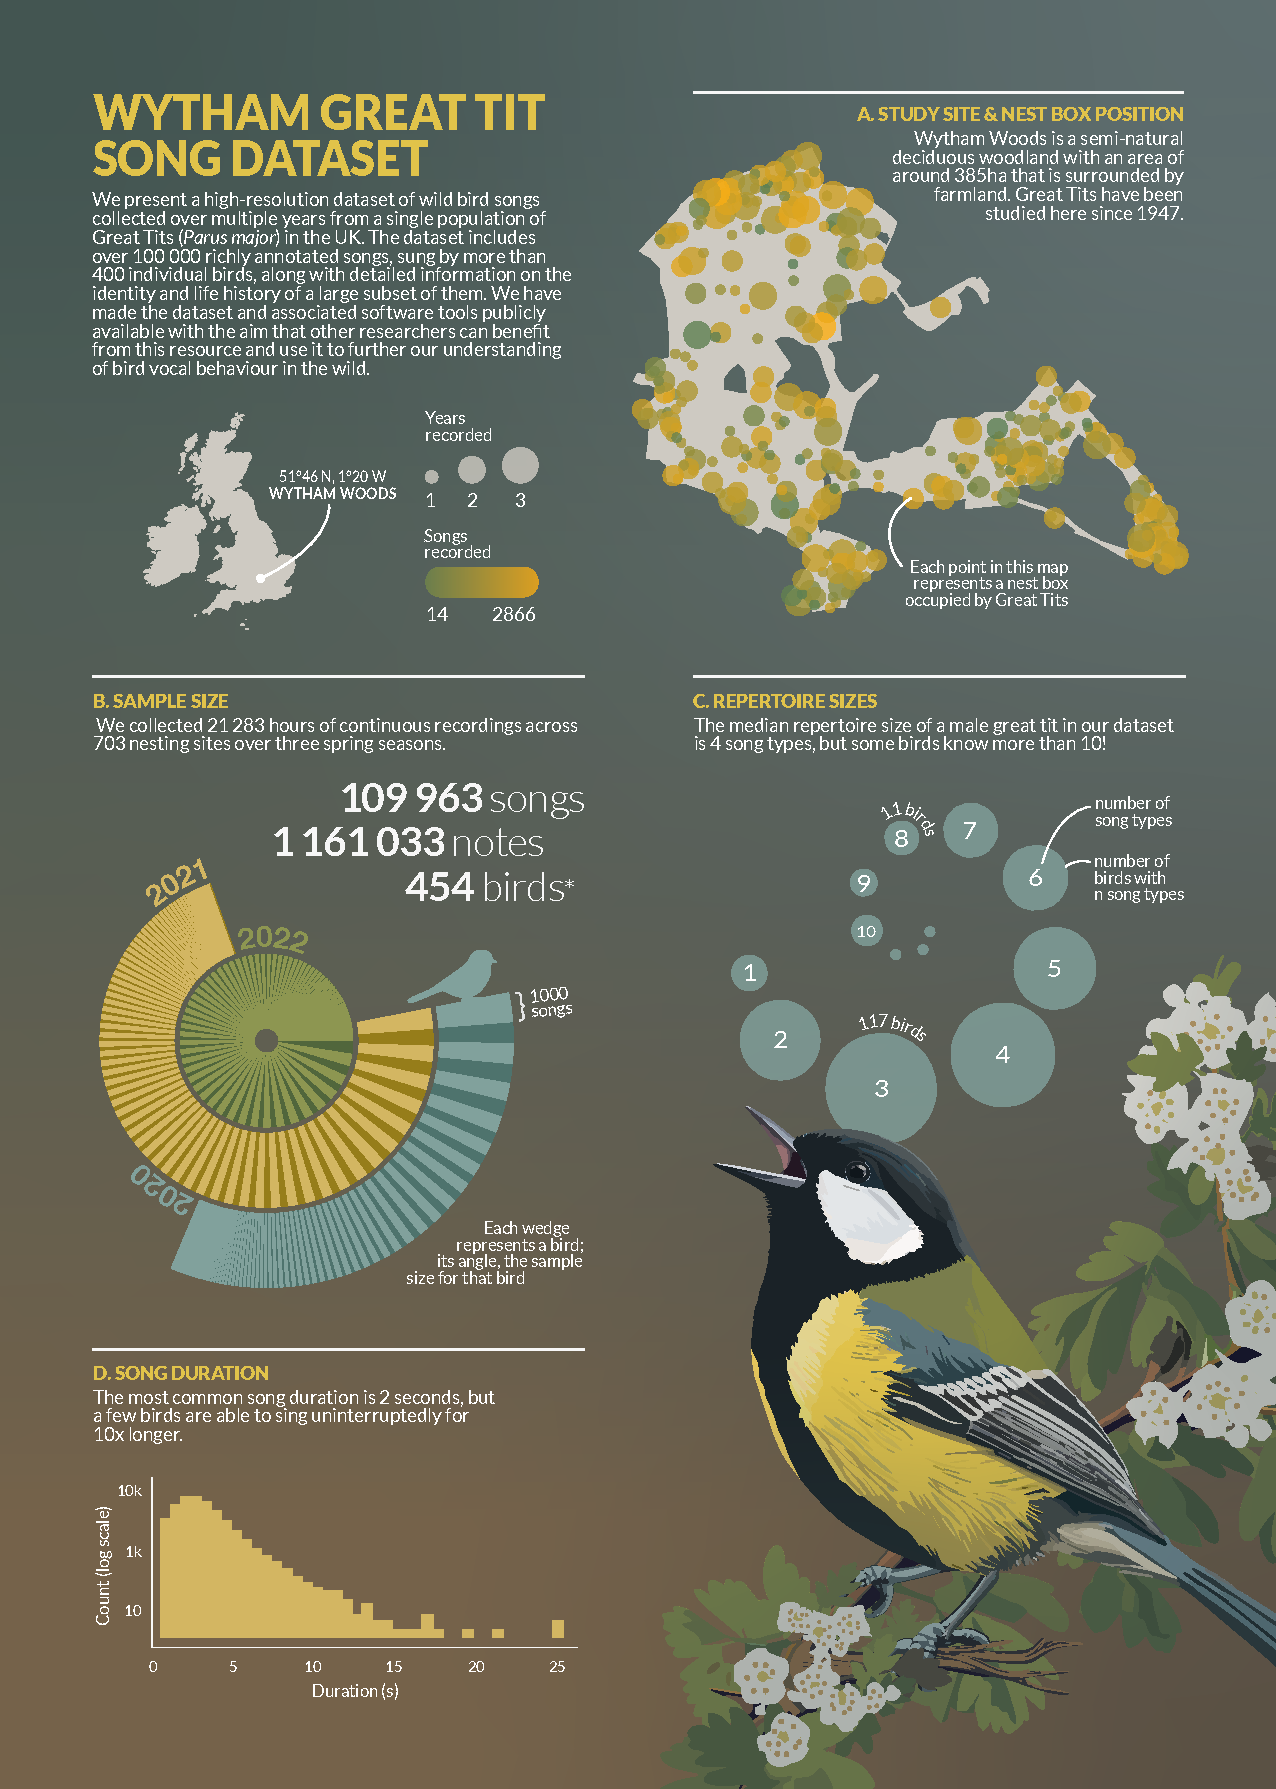
\includegraphics[width=\linewidth]{figures/chapter_3/FIG1-AB.pdf}%
    \mycaption{Description of the study site and dataset}{(A) Map of the study site and sample locations, (B) total sample sizes for each bird and year, (C) distribution of repertoire sizes, and (D) distribution of song lengths. *The exact number of individual birds is not known exactly.}
    \label{c3_fig:summary}
\end{figure*}
%%%%%


In line with this perspective, we present a comprehensive dataset of wild bird songs recorded from a single population of great tits (\textit{Parus major}) in Wytham Woods, Oxford, UK. We collected 21,283 hours of continuous recordings across 703 nesting sites over three spring seasons, which resulted in the annotation of over 1,100,000 notes or acoustic units from more than 100,000 songs (see below for definitions of these terms), sung by approximately 400 different male great tits. Among these birds, we have detailed information on the identity and life history of 242 individuals, including 50 that were recorded in multiple years. This information includes the time and location of breeding attempts, clutch size, number of fledglings, age of the bird, and basic morphological traits. For birds born in the population (106, or 43\% of the total), we also include details such as birthplace, postnatal dispersal distance, mother, and social father. 

To complement the song recordings, we have prepared extensive metadata for each of the more than 100,000 songs. This includes details such as the onset and offset times of each note within the song, a song type label, and the time of recording. We also provide the time of the first song during dawn. Finally, we augment the dataset by providing embeddings of each song, which are vector representations derived from a deep metric learning model specifically trained on this dataset. These can be used to identify individuals and in tasks that require similarity judgements.

Great tit song has been the subject of extensive research activity (see, for example, \cite{lambrechts1990, lind1996, rivera-gutierrez2010a, rivera-gutierrez2010, rivera-gutierrez2011, slagsvold1994, Ritschard2012}). Research conducted within the Wytham Woods population, in particular, has given rise to many influential ideas and insights into bird singing behaviour. These include investigations into neighbour interactions, song matching and the connection between song repertoires and reproductive success \parencite{mcgregor1981, mcgregor1983, mcgregor1989}, the dynamics of song learning from neighbouring individuals and the acquisition of distinct song types \parencite{mcgregor1989, mcgregor1982b}, as well as the role of song repertoires in maintaining territories and reducing listener habituation \parencite{krebs1976, krebs1978}, the functions of dawn song \parencite{kacelnik1983, mace1987}, and the influence of spatial factors and movement on song culture \parencite{fayet2014}. We hope that this dataset---which is, to the best of our knowledge, the largest publicly available collection of bird songs from a single wild population---will contribute to that effort by providing valuable insights into a range of scientific questions, including behavioural repeatability and stability, links between vocal performance and reproductive success, the timing of song production, the syntactic organization of song production, and song learning in the wild.

What follows is a detailed description of the data collection and curation process and the resulting dataset, together with some discussion around potential uses of data presented in this format.

\section{Data collection}
\subsection{Study system \& fieldwork}

Great tits are small, short-lived birds---average lifespan: 1.9 years---that sing acoustically simple yet highly diverse songs. During the breeding season, from March to June, great tit pairs are socially monogamous and defend territories around their nests \parencite{hinde1952}. In Wytham Woods, Oxfordshire, UK (51\degree46 N, 1\degree20 W), a population of these birds has been the focus of a long-term study since 1947 \parencite{lack1964}. Wytham Woods is a semi-natural predominantly deciduous woodland that spans an area of approximately 385 hectares and is surrounded by farmland. Most great tits in this population breed in nest boxes with known locations (see map in \hyperref[c3_fig:summary]{Figure \ref*{c3_fig:summary}}), and the majority of individuals are marked with a unique British Trust for Ornithology (BTO) metal leg ring as nestlings or adults. 

We collected data from late March to mid-May during the breeding seasons of 2020, 2021, and 2022. Every year, fieldworkers checked each of the 1018 nest boxes at least once a week before and during the egg-laying period, which typically lasts from one to 14 days \parencite{Perrins1965}, and recorded the identities of breeding males and females, the dates of clutch initiation and egg hatching, clutch size, and fledgling number and condition under standardized protocols. We found the first egg date by assuming that one egg is laid every day and counting back from the day of observation. In cases where we did not observe the chicks on the day of hatching, the actual hatching date was determined by assessing the weight of the heaviest chicks and extrapolating their age from established growth curves.

To record the vocalizations of male great tits, we took advantage of their behaviour during the reproductive period, when they engage in continuous singing near their nests at dawn before and during egg laying \parencite{mace1987}. Collectively, this vocal display is referred to as the dawn chorus and has been demonstrated to yield a reliable estimation of the song repertoire of individuals when recorded in full \parencite{rivera-gutierrez2012, vanduyse2005}. As soon as we suspected that a pair of great tits were using a nest box based on nest lining materials, egg size if present, or other signs of activity, we deployed an autonomous sound recorder nearby. These recorders were placed on the trunk of the same tree or on a nearby tree, between 1 and 2 metres above the ground and no more than 5 metres away, depending on tree availability. We aimed to keep the recorder in a consistent position and orientation. The microphone pointed upwards and slightly away from the nest box, in the same direction as the entrance hole. The birds sang close to the recorder---we were not able to collect data on this, but the mean distance to the nest box was 10 m in a different population \parencite{halfwerk2012}, which matches our anecdotal observations--- and moved around. Although changes in amplitude due to distance and directionality impacted song selection, we didn't observe any systematic bias.

%%%%% FIG 2: PIPELINE
\begin{figure*}[htbp]
    \centering
    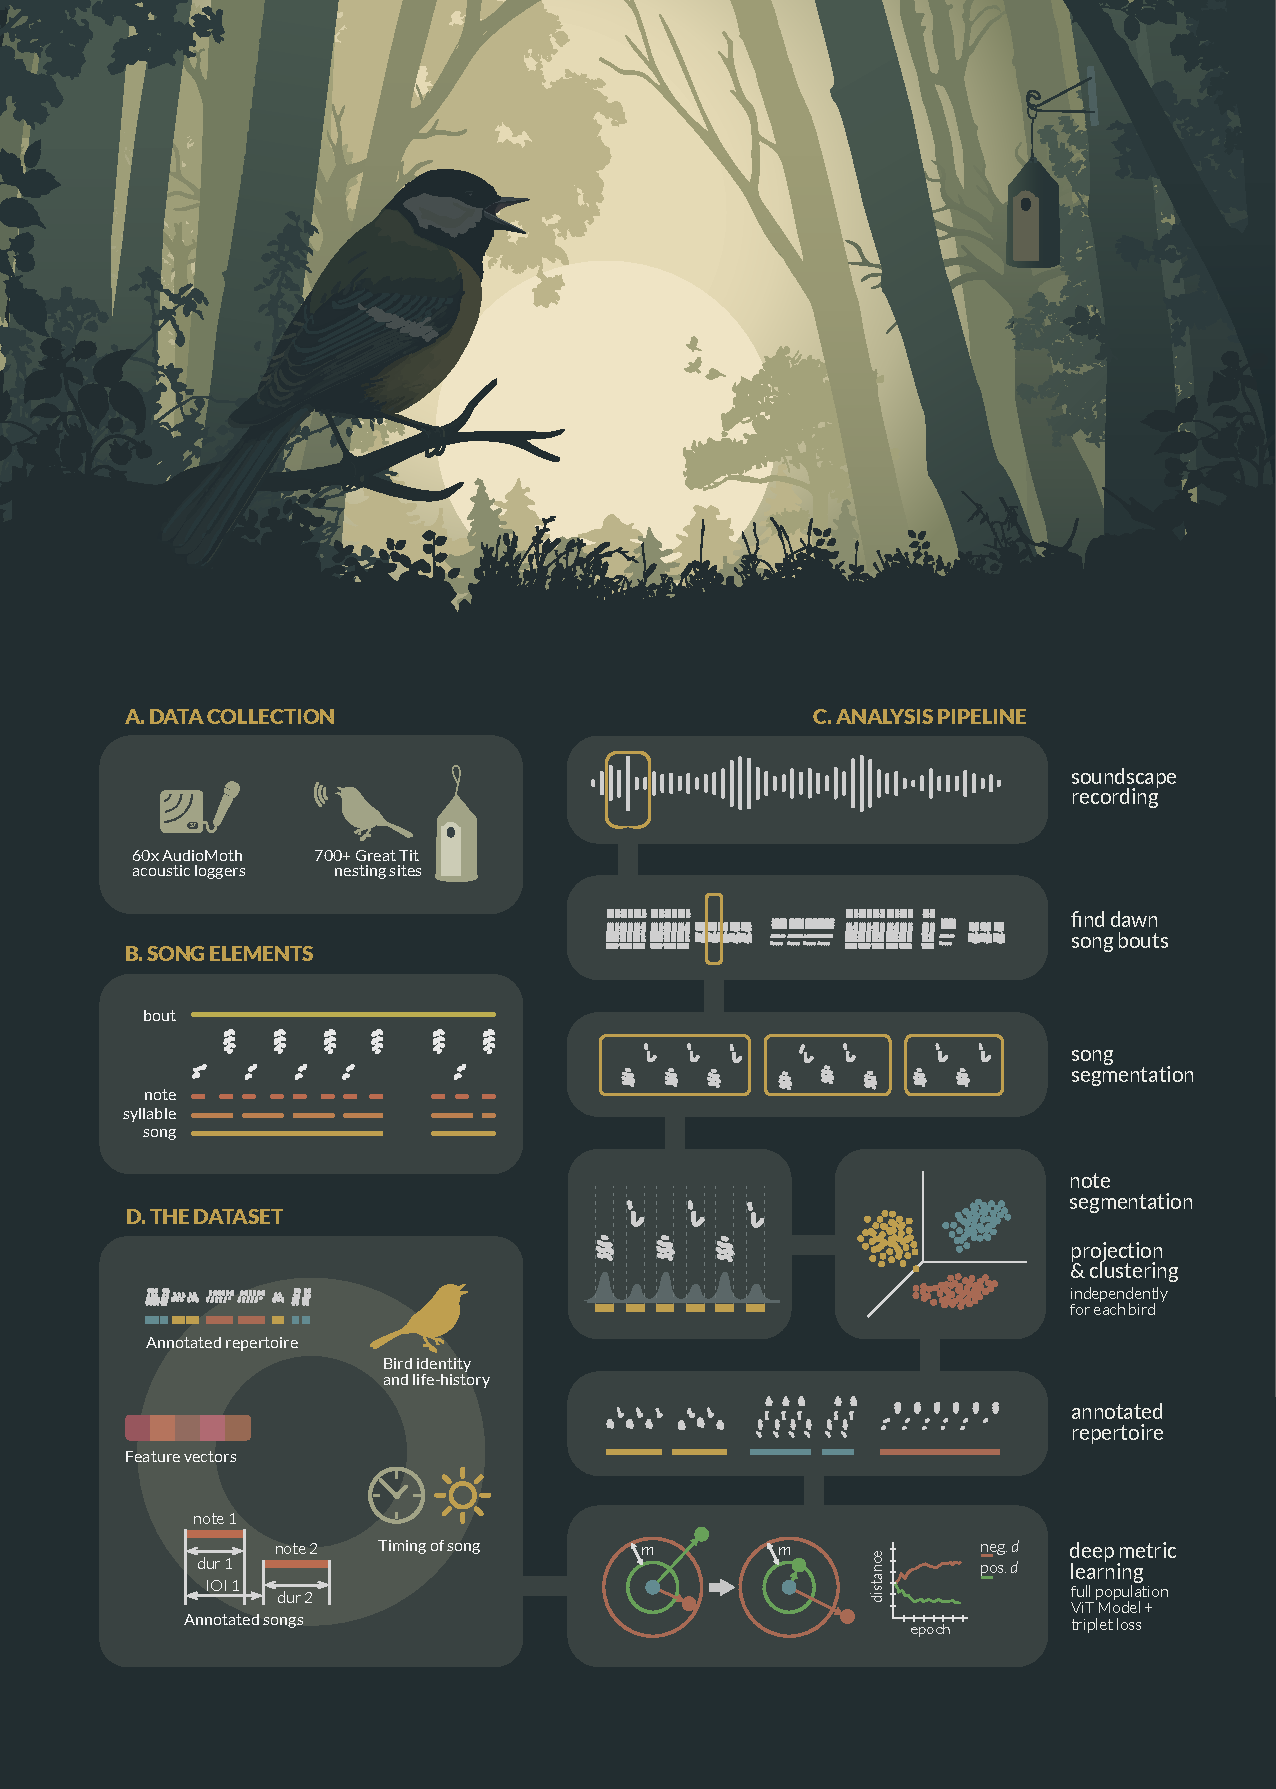
\includegraphics[width=\linewidth]{figures/chapter_3/FIG2-AB.pdf}
    \mycaption{Data collection and analysis pipeline used to prepare the Wytham great tit Song Dataset}{A brief visual summary of the data collection and analysis pipeline used to prepare the Wytham great tit Song Dataset. (A) Data collection in the field. (B) The terminology used to describe the various hierarchical levels at which we can describe great tit's singing. (C) Computational pipeline. (D) Main outputs included as part of the dataset.}
    \label{c3_fig:pipeline}
\end{figure*}
%%%%%

\subsection{Ethical note}
All work involving birds was subject to review by the University of Oxford, Department of Zoology, Animal Welfare and Ethical Review Board (approval number: APA/1/5/ZOO/NASPA/ Sheldon/TitBreedingEcology). Data collection adhered to local guidelines for the use of animals in research and all birds were caught, tagged, and ringed by BTO licence holders.

\subsection{Recording equipment and schedule}

We used 60 (30 in 2020) AudioMoth recorders \parencite{hill2019}, which were housed in waterproof, custom-built enclosures. Recording began approximately one hour before sunrise (05:36 -- 04:00 UTC during the recording period) and consisted of seven consecutive 60-minute-long recordings with a sample rate of 48 kHz, and a depth of 16-bit. To sample as many birds as possible, we left each recorder in the same location for at least three consecutive days before moving it to a different nest box. We relocated 20 recorders (10 in 2020) every day throughout the recording period.

% TODO: theis box causes errors, fix
\begin{tcolorbox}[colback=tablegrey, boxrule=0pt, colframe=white, sharp corners] %TODO: add label here
    \subsection{A note on terminology}
    There is no consistent terminology used to describe the various hierarchical levels of a bird's vocal production. For clarity, we adopt the terminology outlined in \cite{thompson1994}; see also \autoref{c3_fig:pipeline}B for a graphical explanation. 
    \medskip
    The fundamental temporal unit is referred to as a \textbf{note}. Notes are represented by continuous traces on the sound spectrogram and are separated by silences. Moving up the hierarchy, \textbf{syllables} are sequences of one or more notes that are always repeated in the same order. Beyond syllables, we have \textbf{songs}, which consist of clusters of the same type of syllables punctuated by longer pauses, often in the order of seconds. Lastly, song \textbf{bouts} are uninterrupted performances of songs of the same type. great tits tend to sing the same song type repeatedly before transitioning to a different type. They continue this pattern until they stop singing altogether, often after having performed their entire song repertoire.
\end{tcolorbox}

%%%%% FIG 3: QUERIES
\begin{figure*}
    \centering
    \includegraphics[width=\linewidth]{figures/chapter_3/FIG3-AB.pdf}
    \mycaption{A visual representation of the song spectrogram embedding space}{Measuring similarity is a very hard problem, in large part because there is often no objective way to compare the performance of different methods. Here, we took a data-based approach by training a Vision Transformer (ViT) model as a feature extractor in a Euclidean metric learning task. The resulting embedding space allows us to judge if two songs are very similar, and to re-identify birds. (\textbf{A}) PCA projection of the feature vectors: two orthogonal linear components do not capture much of the high-level distinguishing features. (\textbf{B}) This figure shows a UMAP projection of the 384-dimensional vectors for each song in the dataset into 2D, which leads to a fairly arbitrary but useful visualization where tight clusters of points correspond to song types in the repertoire of individual birds. They are coloured by how densely occupied that region of space is in the high-dimensional space, based on k=30 neighbours from other song types. (\textbf{C}) A k-nearest neighbour search returns the closest matches for a query vector (highlighted).}
    \label{c3_fig:queries}
\end{figure*}
%%%%%

\section{Data processing and annotation}

We processed and annotated the recordings using custom software and scripts written in Python 3 \parencite{vanrossum1995}, using the open-source package \texttt{pykanto} \parencite{merinorecalde2023}. These are available from \href{https://github.com/nilomr/great-tit-hits-setup}{\nolinkurl{github.com/nilomr/great-tit-hits-setup}} \parencite{nilo_gretidataset_setup_2023}. \hyperref[c3_fig:pipeline]{Figure \ref*{c3_fig:pipeline}} shows a graphic illustration of the process. See also Box 1 for a note on the terminology used for different parts of the songs.

\subsection{Song segmentation}

We inspected spectrograms for each raw recording and selected songs based on a simple criterion: that its notes were clearly distinct from background noise and other bird vocalizations. We chose entire songs where it was possible; where it was not, we selected the longest contiguous segment possible. This process was carried out manually using the open-source software Sonic Visualizer \parencite{cannam2010} by drawing boxes bounding songs in the time and frequency domains.

\subsection{Assigning song bouts to individuals}

Due to the automated recording process, there is a possibility that some of the recorded songs near a particular nest box may not originate from the focal bird. To minimize the chance of false positives, we discarded recordings with more than one vocalizing bird if one was not distinctly louder than the rest during the segmentation process. Additionally, we discarded all songs with a maximum amplitude below $-16$ dB, calculated as $20 \log_{10}\left(\frac{A}{A_0}\right)$, with $A = 5000$ and $A_0 = 32767$ (the maximum value for 16-bit digital audio). This specific threshold was derived from observations indicating that when simultaneous recordings captured neighbouring birds, an amplitude cut-off greater than 4000 consistently differentiated the focal bird from its closest neighbours. It is important to note that these are not calibrated values and are, therefore, relative to the recording equipment and settings we used --- as well as other factors like sound directionality and vegetation cover.

\subsection{Spectrogramming}

For most operations beyond this point, we used normalized, band-passed and log-scaled mel spectrogram representations of each of the songs (sampling rate = 22050,  window length = 1024, hop length = 128, mel bins = 224; see the repository \href{https://github.com/nilomr/great-tit-hits-setup}{nilomr/great-tit-hits-setup} for full details on the process).

\subsection{Note segmentation}

We segmented the resulting song selections into their constituent notes using a custom dynamic threshold algorithm implemented in pykanto \parencite{merinorecalde2023}, based on the work of \textcite{sainburg2019}. Briefly, the algorithm finds minima in the spectral envelope of a spectrogram, which are considered silences; if the length of the signal between these minima exceeds a maximum note duration, a new local minimum is defined that divides the signal into two shorter segments. This is repeated until multiple notes are defined or there are no local minima below a maximum amplitude threshold. Then, segments below a minimum note duration threshold are discarded. To make the algorithm more robust to noise, the spectrogram is subject to morphological transformations and de-echoing before amplitude information is extracted. The de-echoing algorithm implemented in pykanto is based on that in Luscinia \parencite{lachlan2016a}, and works by subtracting a delayed version of the spectrogram from itself. We determined minimum and maximum note length ranges by manually segmenting a small, random subset of songs (n = 30).

It should be noted that the automated segmentation process is susceptible to various factors that can influence its accuracy. These include background noise, significant variation in amplitude between notes, attenuation caused by vegetation, changes in the direction of sound production, and even variations in performance where some notes may be much quieter. As a result, the algorithm may fail to detect or incorrectly delimit certain notes. Despite this, we estimate that approximately 96\% of the notes are correctly segmented (0.037 error rate based on a random subset of n = 1048 notes that were checked manually). Still, depending on specific goals, we recommend manual verification of note segmentation if complete accuracy is crucial.

\subsection{Song type annotation}

We annotated each song type in the dataset using a semi-supervised approach implemented in \texttt{pykanto}. The process involved several steps to ensure accurate classification. First, we generated average unit spectrograms for each song by taking the mean of the centred and padded spectrograms of its units or notes, which provided a concise representation of the temporal and spectral characteristics of the syllable within it. Next, we performed non-linear dimensionality reduction using UMAP \parencite{mcinnes2018} and a cluster search using HDBSCAN \parencite{mcinnes2017} for each bird in the dataset. See \parencite{sainburg2020a, thomas2021} for similar approaches. This strategy, while useful, often leads to spurious outcomes. For instance, it may separate renditions of the same song type if variation in performance or background noise exists, or if certain song elements are sometimes attenuated. Such variation could be misinterpreted as distinct song types, leading to an overestimation of repertoire size. To address this, we used the interactive app in \texttt{pykanto} to review and split or combine clusters as necessary for each bird. It is worth mentioning that this process would be significantly more challenging in species with highly variable songs: our approach benefited from the great tits' relatively limited repertoires (1 to fewer than 15 song types in our population) and their tendency to produce stable and stereotyped songs.

\subsection{Calculating song embeddings}

Comparing animal vocalizations poses a significant challenge for researchers. Traditionally, two approaches have been used: visual comparisons of spectrograms and, more recently, measurement of hand-picked acoustic features \parencite{goffinet2021}. However, these methods have limitations when dealing with noise, variations in performance, and changes in syntax (where compositional syntax is not relevant). For instance, if a song with the sequence 'tea-cher, tea-cher' is recorded as 'cher-tea, cher', it might be wrongly perceived as highly dissimilar, despite being the same song (see \cite{stowell2021, zandberg2022} for a good overview of these issues). Additionally, these methods often fail to capture high-level features such as the syntactic relationships between notes and other complex spectrotemporal characteristics that cannot be easily characterized by an orthogonal combination of simple acoustic features.

\begin{table*}[ht!]
    \centering
    \mycaption{Short description of the files included in the dataset}{Short description of the files included in the dataset. See \href{https://nilomr.github.io/great-tit-hits}{the docs} for detailed documentation.}
    \label{table:summary}
    \begin{tblr}[
        theme=ntabs
        ]{
        colspec = {X[l]},
        rowsep=3pt,
        stretch = 0.8,
        row{odd} = {tablegrey}, % Shading for odd rows
        cells = {font = \fontsize{8pt}{8pt}\selectfont},
        row{1} = {font=\fontsize{8pt}{8pt}\selectfont} % First row is bold
    }
        109,963 raw song files with their corresponding metadata\\
        Model-based feature vectors, with 109,963 samples and 384 dimensions\\
        A main derived dataset including information on broods, adult bird life-history traits, nesting locations, and acoustic recordings\\
        Morphological measurements for birds captured and re-trapped in the study area. Includes information on species, age, sex, weight, and various other traits\\
        Information on the location and characteristics of nest boxes in Wytham Woods, along with a map of the site\\
    \end{tblr}
\end{table*}

Unfortunately, we cannot rely on the birds' perceptual judgements due to the lack of a hard to obtain experimental data (though recent studies, such as \cite{morfi2021, zandberg2022}, have explored this avenue). This can be an issue where the focus of research is behavioural interactions or the social functions of song. At the same time, for monitoring or individual identification purposes, fully mimicking the bird's perceptual space may not be ideal: the performance of metric learning or classification algorithms trained for narrow purposes can surpass the organism's abilities, as exemplified by facial recognition in humans \parencite{lu2014}. Here, our goal was to define a similarity space based on the inherent variation in the data and the only categorical labels that we know are perceptually and behaviourally significant: song types sung by individual birds. Given that great tits can recognize each other based on their vocalizations \parencite{lind1996}, we aimed to define a similarity space that facilitates similarity-based research and captures some of the song characteristics that birds themselves might attend to when distinguishing individuals. To do this, we took advantage of recent advances in the fields of deep learning and computer vision and used a data-driven approach. Below is a simple narrative description of the process. For further details, see the dedicated repository \href{https://github.com/nilomr/open-metric-learning/tree/great-tit}{nilomr/open-metric-learning} and the OML library \parencite{shabanov2023}. 


\subsubsection{Metric Learning and Vision Transformers}
Rather than focusing on classification, we aimed to develop semantically meaningful embeddings. To achieve this, we used a Vision Transformer (ViT) model as a feature extractor in a (Euclidean) metric learning task. These models, inspired by the success of transformers in natural language processing applications, process images by splitting them into patches, treating them as tokens similar to words in a natural language \parencite{dosovitskiy2021, raghu2022}. In this case, we used the ViT-S/16 architecture (21.7 M parameters), pre-trained on ImageNet using the DINO method (self-distillation with no labels; \cite{caron2021}), and fine-tuned of spectrogram representations of songs.

\subsubsection{Model Training}
During the training phase, we fine-tuned the ViT model using the great tit song dataset. To optimize the performance of the model, we used Triplet loss, a loss function that ensures that the projection of a positive sample, which belongs to the same class as the anchor point (i.e., song-type-within-individual), is closer to the anchor's projection than that of a negative sample, which belongs to a different class, by at least a specified margin \parencite{hermans2017, hoffer2018}. This loss function enables embedding points of the same class to form clusters without collapsing into a single point, which allows us to also explore differences within song types. While training the model we mined hard triplets---where the negative sample is closer to the anchor than the positive---and used the Adam optimizer with a fixed learning rate of $1 \times 10^{-5}$.

\subsubsection{Handling Data Imbalance and Batch Generation}
The distribution of song sample sizes per individual in the great tit dataset approximately follows a power law, resulting in a significant data imbalance. Although the use of triplet loss already addresses this issue to some extent \parencite{thakur2019}, we adopt a random subsampling strategy where classes with more than 100 samples are reduced to 100 for computational efficiency, classes with fewer than 15 samples are excluded to allow a large enough query/gallery split for validation, and we ensure fair representation during training using a balanced sampler \parencite{hermans2017}. Our batch generation strategy involves uniformly sampling P song types without replacement and sampling K spectrograms for each song type, with replication as necessary. This guarantees that all labels are selected at least once in each epoch.

\subsubsection{Train-Time Data Augmentation}
To enhance model robustness and prevent overfitting, we apply various train-time data augmentation techniques \parencite{mumuni2022, perez2017, shorten2019}. These include random cropping in the time domain, dropping out parts of the spectrogram, adding Gaussian and multiplicative noise, equalization, sharpening, changes to brightness and contrast, blurring, and slight shifting in both time and frequency domains. The latter augmentations are applied within the typical variation in performance observed in the great tit vocalizations.

\begin{table*}[ht!]
    \centering
    \mycaption{Description of the dataset and sample sizes}{A brief description of the dataset and sample sizes for different subsets of the data.}
    \label{table:samples}
    \renewcommand{\arraystretch}{0.8}
\begin{tblr}[
    theme=ntabs
    ]{
    colspec = {X[l] X[r]},
    rowsep=2pt,
    stretch = 0.8,
    row{odd} = {tablegrey}, % Shading for odd rows
    cells = {font = \fontsize{8pt}{8pt}\selectfont},
    row{1} = {tableheadgrey, font=\fontsize{8pt}{8pt}\selectfont\bfseries}, % First row is bold
}
    Description                                           & Value                \\
    Number of segmented notes                             & 1,161,033            \\
    Number of songs                                      & 109,963              \\
    Mean repertoire size                                 & 4.24                 \\
    SD repertoire size                                   & 1.98                 \\
    Median repertoire size                               & 4                    \\
    Number of unique classes                             & 1,930                \\
    Mean class size                                      & 56.98                \\
    SD class size                                        & 68.35                \\
    Median class size                                    & 31                   \\
    Number of nest sites recorded                        & 706                  \\
    Number of nest sites with data                       & 454                  \\
    Number of unique birds with data that were ID'd      & 242                  \\
    Number of times each bird was recorded               & 192 (1y), 42 (2y), 8 (3y) \\
\end{tblr}
\end{table*}

\subsubsection{Results}
Our trained model shows very good performance, achieving a mean Average Precision at 5 (mAP@5) of 0.98 and a Cumulative Matching Characteristic at 1 (CMC@1) of 0.98. This indicates that in approximately 98\% of the queries made to the similarity space, the returned candidate song type by a bird is the correct one. Errors primarily stemmed from instances where songs of the same type sung by the same bird appeared more than once in the dataset, which happened if a bird survived to the next year. Given that the model was trained on almost 2000 classes, this means that there is enough individual information contained in each song type to distinguish between birds with high confidence, which has important implications for both the study of individuality and population monitoring. See \hyperref[c3_fig:queries]{Figure \ref*{c3_fig:queries}} for a visual representation of the embedding space and nearest-neighbour queries.

\section{Data records and description}

\hyperref[table:summary]{Table A\ref*{table:summary}} contains a summary of the files included with the dataset. Detailed data documentation, including variable descriptions, can be found online at \href{https://nilomr.github.io/great-tit-hits/}{nilomr.github.io/great-tit-hits}.

The dataset provides a comprehensive view of the populations' natural dawn singing behaviour over three spring seasons. It documents changes in individual performance, the appearance and disappearance of birds---and with them, their songs---and highlights just how much behavioural variation there is along every dimension of what could at first seem a relatively simple trait. \hyperref[table:samples]{Table \ref*{table:samples}} presents some simple summary statistics, and \hyperref[c3_fig:summary]{Figure \ref*{c3_fig:summary}} provides a visual overview of the dataset.

Even though most birds in the dataset are one or two-year-olds recorded within a single year (which can be attributed to high turnover rates in the population given low annual survival), the dataset includes valuable data on much older individuals, including a 7-year-old. Among the recorded birds, some display metronome-like regularity in their performance, while others have highly variable or unusual songs, due to learning from allospecific vocalizations, or even issues with their vocal apparatus. You can find some interactive examples at \href{https://nilomr.github.io/great-tit-hits/}{nilomr.github.io/great-tit-hits}. The longest song recorded is approximately 20 times longer than the shortest song (and, coincidentally, was sung by one of the largest great tits ever recorded in the Wytham population). The median number of songs per song type and per bird in the dataset is 31, with a significant number of birds having a much larger count, reaching into the thousands; the median repertoire size per bird is four song types, although some birds performed as many as 13 distinct song types.

\subsection{Known biases and problems}

Working with third-party datasets can be challenging, perhaps particularly so in the study of behaviour in natural populations. The familiarity that fieldworkers inevitably develop with the study system and the data is difficult to replace, and, as a result, there is a risk of unintentionally overlooking important sources of bias and variability. We have compiled a list of some key considerations, which, while not exhaustive, can serve as a starting point for identifying and addressing biases when testing hypotheses, estimating parameters, or evaluating findings from the data. These issues can be broadly classified into two groups: those around bird and song type labelling, which can be partially addressed, and those that are inherent in the data or how it was collected.


\subsubsection{Individual and song identification}

One factor that can be partially addressed is that the birds recorded in our dataset are not a random subset of the population; they are those that establish territories and begin the breeding process. In turn, birds that are subsequently identified are more likely to be those whose chicks hatch and survive for at least six days, when the first identification attempt is made. This may skew the distribution of certain behaviours within the dataset or lead to endogenous selection bias \parencite{elwert2014}. One way to quantify the extent to which the subset of identified birds is representative of the entire breeding population would be to compare the distribution of the trait of interest in both groups. See, for example, \cite{kidd2015}, who found that females in nests that fail early in our population are more likely to be immigrant birds breeding in poor-quality areas.

Another issue to consider is that birds may attempt to breed again in the same nest box or elsewhere after a failed attempt. This, coupled with a failure to identify the male associated with those attempts, means that it is conceivable (although likely very rare) that songs from the same bird could appear in the same year twice, leading to pseudoreplication. Similarly, unidentified birds present in the dataset for multiple years could contribute to this problem. One potential way to address these issues is by using song embeddings for identification based on similarity and assigning dummy IDs to birds believed to be the same individual. At least, this should be modelled to assess the sensitivity of any results to varying degrees of pseudoreplication from this source.

Finally, a few songs might have been mislabelled before model training, as it is not feasible to manually check such a large dataset. However, the model-based embeddings can help identify any mislabelled songs: they will be clear outliers within their respective classes, thanks to the relatively discrete nature of great tit repertoires.


\subsubsection{Unequal samples; songs and calls---and female song}

As is common in many complex systems, the interaction of the many processes involved in both song production and sampling results in a heavy-tailed frequency distribution of sample sizes. This variation stems from various sources, including characteristics inherent to the study system, such as individual differences in singing activity and temporal fluctuations throughout spring. The sampling process introduces further variation, through factors like equipment malfunctions causing small gaps in the data, variation in recording dates relative to peak activity, and the impact of rain and hail on singing activity and recording quality. We cannot assume these processes to be completely independent of each other. Therefore, when analysing song output or repertoire size, it is important to explicitly specify the assumed causal relationship between factors such as individual characteristics, sampling probability, and the outcome measure.

Another important aspect to consider is that, while we have said that the dataset consists of songs, the demarcation between songs and calls is not entirely straightforward. Some vocalizations that would typically be classified as calls, due to their acoustically simpler, shorter, and possibly more stereotyped nature, are actually used as part of the dawn vocal behaviour. These vocalizations are repeated in a manner that creates an impression of functional equivalence to songs. While we have followed criteria similar to other studies \parencite{baker1986, fayet2014, krebs1978, rivera-gutierrez2010a} to maintain consistency, we believe that this phenomenon warrants further attention. These calls were not segmented and thus are not included in the dataset, but we are happy to provide soundscape recordings to anyone interested in exploring this aspect further.

Finally, although female song in birds has received relatively little historical attention (see \cite{langmore2020, odom2018, riebel2005} for further discussion), female great tits also sing (see a brief treatment in \cite{gompertz1961, hinde1952}). The vast majority of songs in the dataset belong to the dawn song, a behaviour exclusively performed by the male prior to the female leaving the nest (a pattern observed in blue tits as well, as documented by \cite{sierro2022}). Females, on the other hand, vocalize within the nest, but these vocalizations \parencite{gorissen2005, gorissen2004} differ from songs and were not typically detectable by our recording devices. Nevertheless, \cite{hinde1952} suggests that in the absence of males, females may be more inclined to engage in territorial behaviour that involves singing rather than just producing calls. If that is the case, it is possible that our dataset contains some isolated instances of female song.

%%%%% FIG 4: 
\begin{figure*}[th!]
    \centering
    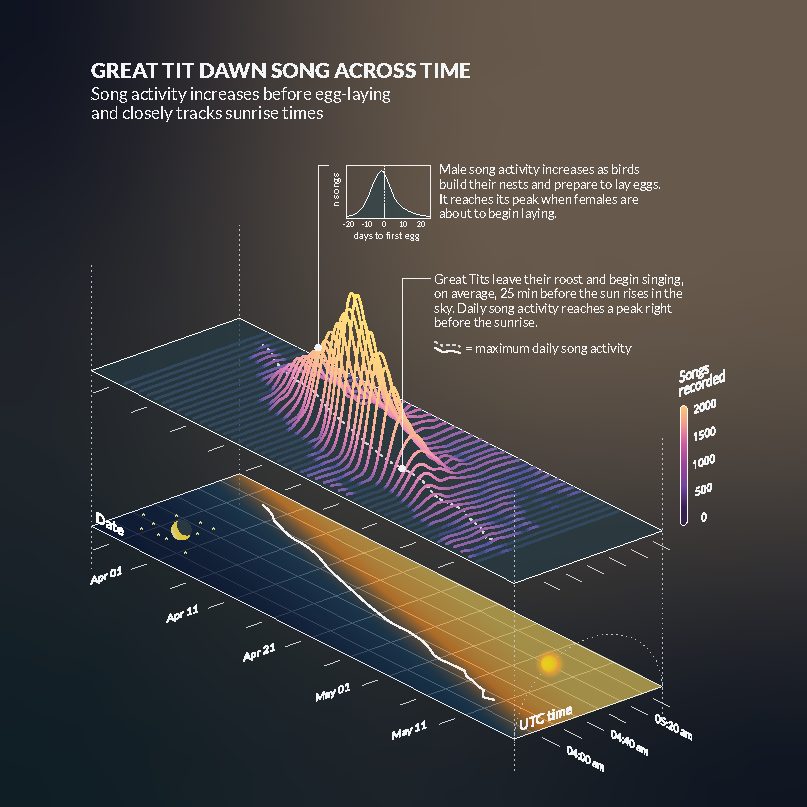
\includegraphics[width=\linewidth]{figures/chapter_3/FIG4-AB.pdf}
    \mycaption{Great tit song activity closely tracks advancing sunrise times and female fertility}{Days get longer as the spring progresses and male great tits track the advancing sunrise times with great precision, so that they always begin singing, on average, 25 minutes before the morning breaks. This figure also shows (z-axis) how song activity peaks alongside egg laying: males sing the most in the morning right before their partner lays the first egg.}
    \label{c3_fig:timing}
\end{figure*}
%%%%%

\section{Uses and suggestions}

The dataset we are presenting contains detailed information about the vocal behaviour and life of wild birds, providing valuable opportunities for investigating a wide range of research questions. In this section, we suggest several research areas that can be explored using this dataset and provide references to relevant studies in the literature.

\textbf{Behavioural repeatability and stability across multiple scales}: Researchers can use the dataset to examine the repeatability and stability of song production and song characteristics across different temporal and spatial scales. This includes studying consistency in vocal behaviour within individuals over time and across different contexts, and its links to age \parencite{rivera-gutierrez2012, zipple2019} and reproductive fitness \parencite{sierro2023}.

\textbf{Links between vocal performance or diversity and reproductive success}: Our data can be used to explore the relationships between vocal performance metrics, such as song complexity or vocal diversity, and individual breeding success on a dataset that is much larger than what is typical in the field \parencite{hutfluss2022, beecher2020a, crates2021, hiebert1989, mcgregor1981}. 

\textbf{Spatial and temporal properties of acoustic communities}: The dataset enables investigations into the spatial properties of acoustic communities, including the distribution of singing individuals within a given habitat and across time. This can provide valuable insights into the spatial dynamics of communication networks and acoustic interaction among neighbour birds.

\textbf{Timing and volume of song production}: Researchers can use the dataset to analyse the temporal patterns and timing of song production in great tits. This might involve studying diurnal variation, seasonal trends, and the influence of environmental factors on the timing and abundance of vocal behaviour. As an example, \hyperref[c3_fig:timing]{Figure \ref*{c3_fig:timing}} provides an overview of key temporal shifts in dawn singing behaviour: male birds sing more during the fertile period of the female, and their activity closely tracks advancing sunrise times.

\textbf{The syntactic organization of song production}: The dataset captures song activity over entire dawn song periods, across days, and even years for many individuals. This would allow researchers to investigate the set of rules that govern the arrangement of song elements and transitions within the vocal repertoire of wild great tits, in terms of short and long-distance dependencies and other properties of their sequential dynamics \parencite{hedley2018, lachlan2010, sainburg2019, searcy2022}.

\textbf{Song learning in the wild}: While this dataset does not directly provide evidence of song learning, researchers can use song similarity and proximity in time and space to infer cultural transmission processes. This allows for the exploration of the influence of spatial and social factors on song learning \parencite{james2020, lachlan2003, nelson2014, peters2017, wheelwright2008}.


\section{Conclusion}

With over 1,100,000 annotated notes and acoustic units from more than 100,000 songs, collected over three spring seasons, we hope that this dataset will offer valuable insights into bird vocal behaviour and song culture. The dataset is enriched with detailed metadata such as note onset and offset times, song type labels and embeddings derived from a deep metric learning model, as well as identity and life-history information for the birds, which makes it useful for a wide range of research purposes. By sharing this comprehensive dataset, we also aim to help promote data-sharing and scientific collaboration.

\section{Author contributions}

LP, AV, AE and NMR collected the data. NMR created the software and pipeline to plan fieldwork and analyse the data, annotated the dataset with help from AE, built the website, documentation, and visualizations, and wrote the original draft. BCS and EFC provided feedback and supervision throughout the research, and all authors contributed critically to drafts.

\section{Acknowledgements}
We thank all those who have contributed to the long-term nest box study in Wytham Woods and the collection of associated data.
This work was supported by a Clarendon-Mary Frances Wagley Graduate Scholarship
and an Edward Grey Institute scholarship to Nilo Merino Recalde and made use of the University of Oxford Advanced Research Computing facility \parencite{richards2015}.

\section{Conflict of interest statement}
The authors declare no conflict of interest.

\section{Data and code: availability and use}

The complete Wytham great tit Song Dataset and its metadata are available at \href{https://osf.io/n8ac9/}{\nolinkurl{10.17605/OSF.IO/N8AC9}} \parencite{nilo_gretidataset_osf_2023}. The code to train the deep metric learning model can be found at \href{https://github.com/nilomr/open-metric-learning/tree/great-tit}{nilomr/open-metric-learning}. See the \href{https://nilomr.github.io/great-tit-hits/}{dataset website} for documentation and more information.

All input and output data files use open data formats and are under a \href{https://creativecommons.org/licenses/by/4.0/}{CC-BY-4.0} licence. The scripts and software used to create this dataset are available under the \href{https://github.com/nilomr/pykanto-example/blob/main/LICENSE}{MIT} licence from GitHub \href{https://github.com/nilomr/great-tit-hits-setup}{nilomr/great-tit-hits-setup} and archived at Zenodo \parencite{nilo_gretidataset_setup_2023}.

\renewcommand{\cleardoublepage}{}
\renewcommand{\clearpage}{}
\printbibliography
